% Options for packages loaded elsewhere
\PassOptionsToPackage{unicode}{hyperref}
\PassOptionsToPackage{hyphens}{url}
\PassOptionsToPackage{dvipsnames,svgnames,x11names}{xcolor}
%
\documentclass[
  10pt,
  dvipsnames, enabledeprecatedfontcommands]{scrartcl}
\usepackage{amsmath,amssymb}
\usepackage{lmodern}
\usepackage{iftex}
\ifPDFTeX
  \usepackage[T1]{fontenc}
  \usepackage[utf8]{inputenc}
  \usepackage{textcomp} % provide euro and other symbols
\else % if luatex or xetex
  \usepackage{unicode-math}
  \defaultfontfeatures{Scale=MatchLowercase}
  \defaultfontfeatures[\rmfamily]{Ligatures=TeX,Scale=1}
\fi
% Use upquote if available, for straight quotes in verbatim environments
\IfFileExists{upquote.sty}{\usepackage{upquote}}{}
\IfFileExists{microtype.sty}{% use microtype if available
  \usepackage[]{microtype}
  \UseMicrotypeSet[protrusion]{basicmath} % disable protrusion for tt fonts
}{}
\makeatletter
\@ifundefined{KOMAClassName}{% if non-KOMA class
  \IfFileExists{parskip.sty}{%
    \usepackage{parskip}
  }{% else
    \setlength{\parindent}{0pt}
    \setlength{\parskip}{6pt plus 2pt minus 1pt}}
}{% if KOMA class
  \KOMAoptions{parskip=half}}
\makeatother
\usepackage{xcolor}
\usepackage{graphicx}
\makeatletter
\def\maxwidth{\ifdim\Gin@nat@width>\linewidth\linewidth\else\Gin@nat@width\fi}
\def\maxheight{\ifdim\Gin@nat@height>\textheight\textheight\else\Gin@nat@height\fi}
\makeatother
% Scale images if necessary, so that they will not overflow the page
% margins by default, and it is still possible to overwrite the defaults
% using explicit options in \includegraphics[width, height, ...]{}
\setkeys{Gin}{width=\maxwidth,height=\maxheight,keepaspectratio}
% Set default figure placement to htbp
\makeatletter
\def\fps@figure{htbp}
\makeatother
\setlength{\emergencystretch}{3em} % prevent overfull lines
\providecommand{\tightlist}{%
  \setlength{\itemsep}{0pt}\setlength{\parskip}{0pt}}
\setcounter{secnumdepth}{-\maxdimen} % remove section numbering
\usepackage{booktabs}
\usepackage{longtable}
\usepackage{array}
\usepackage{multirow}
\usepackage{wrapfig}
\usepackage{float}
\usepackage{colortbl}
\usepackage{pdflscape}
\usepackage{tabu}
\usepackage{threeparttable}
\usepackage{threeparttablex}
\usepackage[normalem]{ulem}
\usepackage{makecell}
\usepackage{xcolor}
\ifLuaTeX
  \usepackage{selnolig}  % disable illegal ligatures
\fi
\IfFileExists{bookmark.sty}{\usepackage{bookmark}}{\usepackage{hyperref}}
\IfFileExists{xurl.sty}{\usepackage{xurl}}{} % add URL line breaks if available
\urlstyle{same} % disable monospaced font for URLs
\hypersetup{
  pdftitle={Volunteers in NESTA experiment Technical Report},
  pdfauthor={Rafal Urbaniak},
  colorlinks=true,
  linkcolor={Maroon},
  filecolor={Maroon},
  citecolor={Blue},
  urlcolor={blue},
  pdfcreator={LaTeX via pandoc}}

\title{Volunteers in NESTA experiment \linebreak  Technical Report}
\author{Rafal Urbaniak}
\date{}

\begin{document}
\maketitle

The winning model, given our model selection method, is specified as
follows:

\begin{align*}
\mathsf{interventions} \sim \mathsf{NegativeBinomial} (\lambda,\phi) \\
log(\lambda) = l_\mathsf{volunteerID[i]} + enth_\mathsf{ volunteerID[i]} \times \mathsf{daysOfProject} + comp_\mathsf{volunteerID[i]} \times \mathsf{competition}\\  
l_\mathsf{ volunteerID[i] }  \sim \mathsf{Norm}(lbar,lsigmabar) \\
lbar \sim \mathsf{Norm}(2, .9)\\
lsigmabar, enthsigmabar, compsigmabar \sim  \mathsf{Exp}(.5) \\
enth _\mathsf{ volunteerID[i] }  \sim \mathsf{Norm}(enthbar, enthsigmabar)\\
comp_\mathsf{ volunteerID[i] } \sim \mathsf{Norm}(compbar, compsigmabar) \\
enthbar, compbar \sim  \mathsf{Norm}(0, .3)\\
 \phi =  puser_\mathsf{ volunteerID[i] }  \\
 puser_\mathsf{ volunteerID[i] } \sim \mathsf{Exp}(1)
\end{align*}

Intuitively, volunteer interventions are assumed to have negative
binomial distribution around their own expected value \(\lambda\) and
individualized dispersion parameters \(\phi\). On each day each a user
has their own daily expected value, which is determined by the following
factors:

\begin{itemize}
\item First, there's user's individual baseline activity for the whole treatment period, $l_\mathsf{ volunteerID[i] }$.
\item next, each user has their own dispersion parameter,  $puser_\mathsf{ volunteerID[i] }$.
\item then, there is (usually dwindling) enthusiasm: the impact of time on that user, $enth_\mathsf{volunteerID[i]} $ to be (after exponentiation) multiplied by the number of days that have passed since the experiment started,
\item finally, we have the impact that the presence of competitions made on a user, $comp_\mathsf{ volunteerID[i] }$, which (after exponentiation) becomes the activity multiplier to be applied during competitions only.
\end{itemize}

\noindent Moreover, the model is hierarchical: the individual level
parameters are drawn from distributions whose parameters are in turn to
be estimated as well. Thus, \(lbar\) is the overall baseline for the
whole group, \(enthbar\) is the overall estimated group enthusiasm
coefficient, and \(compbar\) is the overall estimated competition impact
coefficient (all of them come with their own nuisance sigma parameters).

\noindent All of these parameters are given priors in a manner analogous
to the introduction of priors for the other time series models, as
explained in the appendix.\footnote{Interestingly, if we are interested
  in the causal effect of competitions, we should not use an
  auto-regressive predictor. If we auto-regress on a lag in the
  \([1,7]\) range, for some days we will be conditioning on
  interventions conducted during the same competition, which will
  already contain some information about the impact of that competition.
  In other words, auto-regression with short lags would lead to
  post-treatment bias. On the other hand, auto-regression with longer
  lags would either lead to dropping a lot of data in the beginning
  (where lagged information is not available), or degenerate the
  analysis by using 0s for missing lagged values in a long initial
  period. All this without much gain, as we have already inspected null
  models with auto-regression with large lags and they do not lead to
  performance improvement.}

Raw data and daily means are illustrated in Figure
\ref{fig:volunteersBasic}, and the individualized totals with the key
coefficients based on the trained model are illustrated in Figure
\ref{fig:volunteersModel}.

\begin{figure}

\begin{center}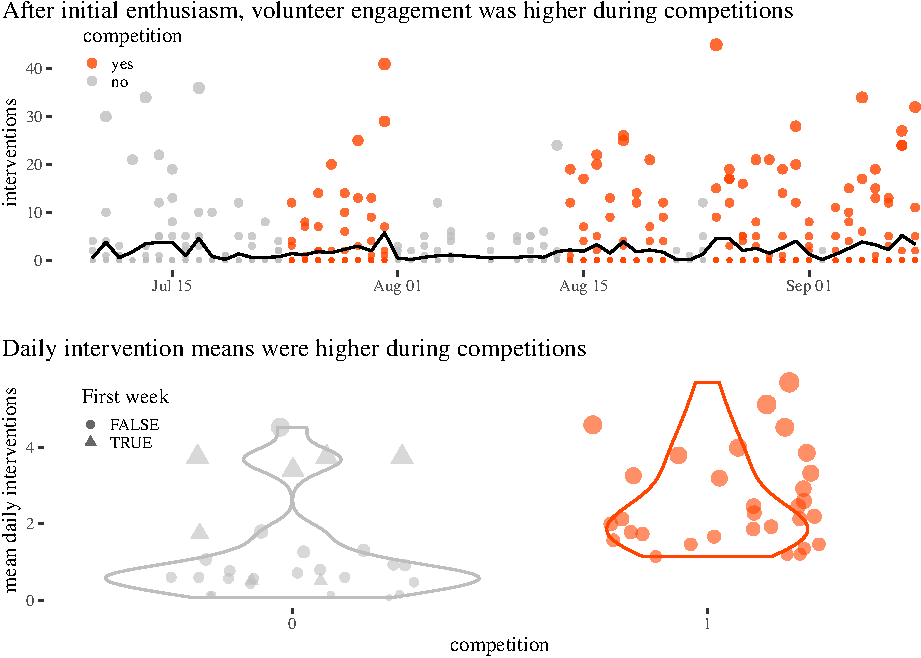
\includegraphics[width=1\linewidth]{reportVolunteers_files/figure-latex/fig:volunteersBasic5-1} \end{center}
\caption{Daily individual voilunteer intervention counts accross time with competition periods marked (top) and daily group intervention means grouped by whether a competition was ongoing (bottom). Note most of high means in the non-competition period are in the first week.}
\label{fig:volunteersBasic}
\end{figure}

\begin{figure}

\begin{center}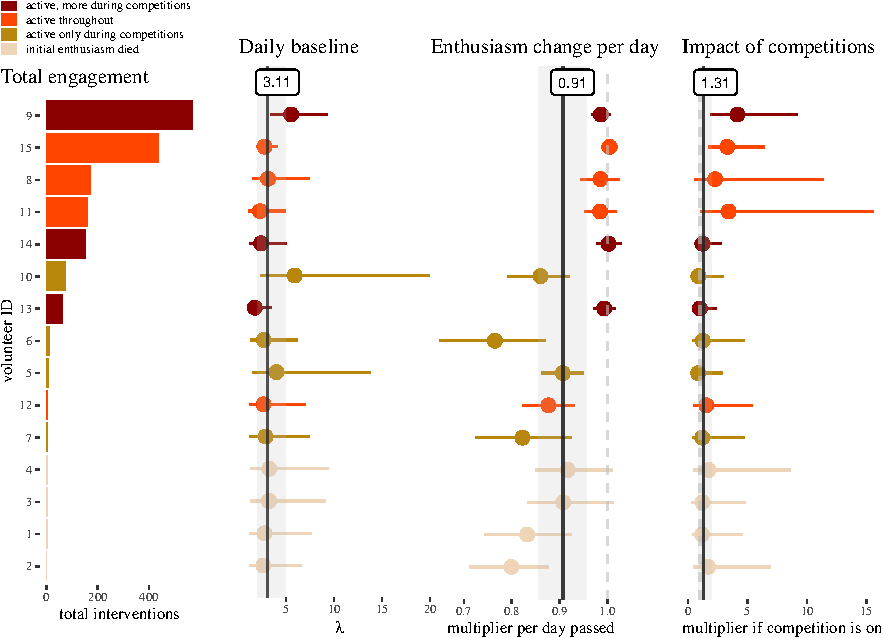
\includegraphics[width=2.5\linewidth,angle=90]{reportVolunteers_files/figure-latex/fig:volunteersModel17-1} \end{center}
\caption{Volunteer total engagement with their daily baseline and multipliers for enthusiasm and impact of competition. Pointranges represent individual level coefficients, group coefficients are represented by black lines with shaded 89\% HPDI areas.}
\label{fig:volunteersModel}
\end{figure}

\end{document}
